No momento em que a tela retratada na \autoref{fig:drAPIorder} inicia, um serviço de consulta para capturar informações do pedido requerido é executado. Esse serviço realiza uma requisição \textit{GET} na rota \textit{/order/\{id\}}, parametrizada para receber o código do pedido no estabelecimento, integrado pelo sistema anteriormente.

Nesse momento os possíveis status do pedido poderem ser: 
\\ \textit{INTEGRATED}, \textit{CANCELLED}, \textit{DISPATCHED}, \textit{DELIVERED} ou \textit{CONCLUDED}.

\begin{figure}[H]
    \centering
    \caption{Delivery Routes - API - order}
    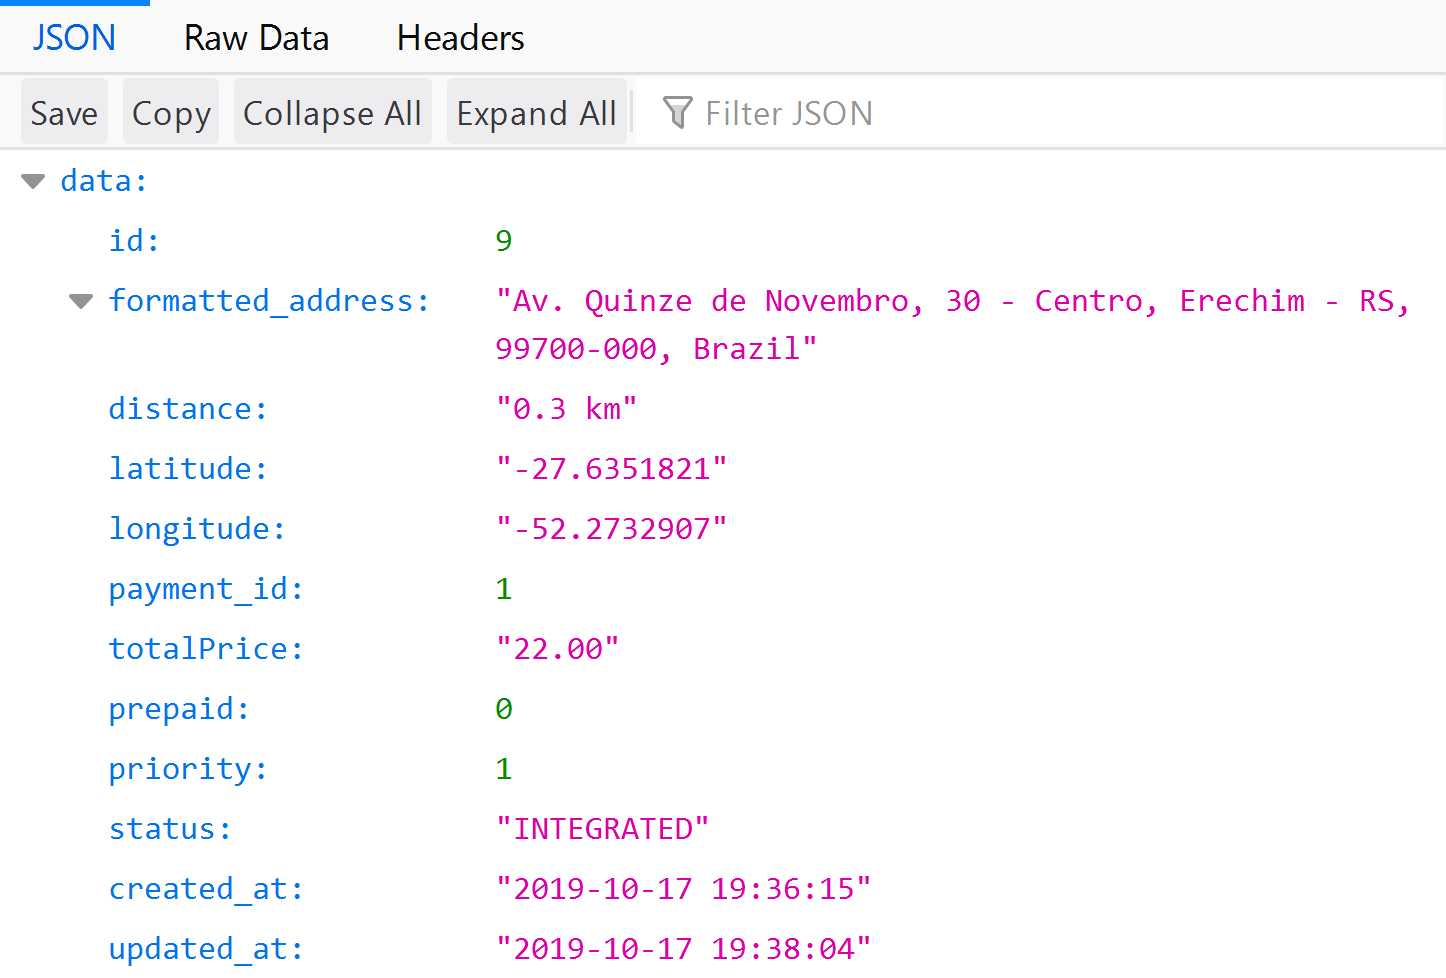
\includegraphics[width=0.9\textwidth]{./dados/figuras/fig22}
    \fonte{Autor}
    \label{fig:drAPIorder}
\end{figure}

Como resultado dessa consulta (como demonstra o \autoref{alg:getOrder}), o servidor retorna o objeto requisitado (em formato JSON) com os respectivos dados solicitados pela rota, por meio da ferramenta  \textit{Resources}, exercendo a sua função como um camada de tratamento entre o Eloquent ORM e as respostas JSON que são expostas pela API. Essas classes, criadas ao executar o comando \textit{php artisan make:resource OrdersResource} através do Artisan, permitem transformar facilmente, \textit{models} e \textit{collections} em JSON.

\begin{lstlisting}[caption={Delivery Routes - Route order}, style=htmlcssjs, label=alg:getOrder]
Route::get('/order/{id}', function ($order_id) {
    return new OrdersResource(Order::find($order_id));
});
\end{lstlisting}